\chapter{WW Scattering}
\section{Introduction}
When two W-boson interacts directly it is known as WW scattering. It is shown in figure \ref{wwscattering1}.
\begin{figure}[htb]
	\begin{center}
		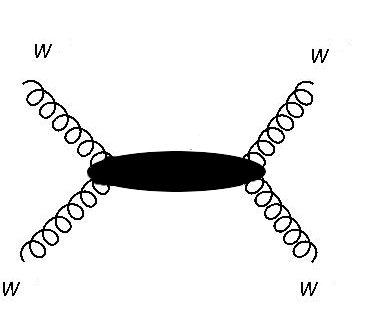
\includegraphics[width=8.0cm,height=6cm]{figures/VBS/H-mediated.png}
		\caption{WW scattering process}
		\label{wwscattering1}
	\end{center}
\end{figure} 
In figure black box represent that we do not know the process by which it is happening. It may be the Higgs which is responsible for it or may be something else which is beyond standard model scenario.
\section{Motivation for WW Scattering}
In July 2012, a new Higgs like particle was discovered with mass $125.7\pm 0.3(stat)\pm 0.3 (syst)$ GeV at the LHC \cite{paper:Higgs2013}. This may be the long sought Higgs boson of the {sm}, which was proposed in 1960s, or one of the Higgs bosons beyond the {sm} predicted by many BSM models. For example, super-symmetric theories, little-Higgs models, and other extended Higgs sector such as the two-Higgs-doublet model (2HDM) all contain a multitude of neutral as well as charged Higgs bosons\cite{paper:13036335v1}. Because, the statistical and systematic uncertainties of current data are still sizable ($\sim20\%$ in the best cases), therefore it is not possible at present to conclude with precision whether this particle is the Higgs boson of the {sm}, nor if new physics is present in the Higgs sector\cite{paper:Higgs2013}.

A well known probe to {ewsb} is the scattering of the longitudinal components of the weak gauge bosons\cite{paper:13036335v1}.% The scattering amplitude with purely gauge contributions grow with energy as $s/m^2_w$, where s is the squared  \gls{com} energy of the $W_LW_L$ system. In the SM with light Higgs boson, the amplitude will be completely unitarized by the Higgs boson. Once $\sqrt{s}$ goes beyond the light Higgs boson mass, the scattering amplitude will no longer grow like $s/m^2_w$. 
The centrality of WW scattering to the exploration of {ewsb} stems from the issue of cancellation of high energy divergences. Any scattering amplitude in a consistent quantum mechanical theory must respect the unitarity, which is equivalent to the conservation of total probability. This implies that no amplitude can indefinitely grow with energy. The reaction which best exemplifies the relationship between unitarity and {ewsb} is the scattering among longitudinally polarized vector bosons. The Feynman diagrams for $W^+W^-\rightarrow W^+W^-$ are shown in Figure \ref{wwscattering} \cite{report:wwscatering}.% The polarization vectors of a transversely/longitudinally (T/L) polarized W boson travelling along the $\hat{z}$ axis are:
\begin{figure}[htb]
	\begin{center}
		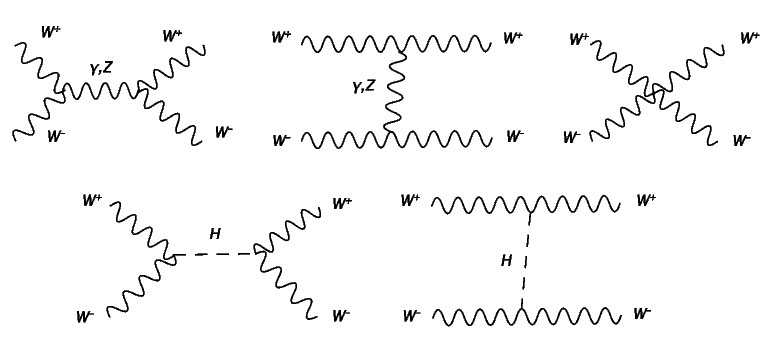
\includegraphics[width=14.0cm,height=8cm]{figures/VBS/wwscattering.png}
		\caption{Vector boson scattering process}
		\label{wwscattering}
	\end{center}
\end{figure} 

%In WW scattering, in the absence of a relatively light Higgs boson, treelevel unitarity is violated at about 1 TeV, therefore either the Higgs must exist or some other mechanism must intervene at about the TeV scale and play same role in taming the divergent behaviour of high energy amplitudes. Hence these processes are the ideal testing ground for the mechanism of EWSB.

\begin{comment}
So, It is important to at-least constraint the various couplings of the Higgs boson, based on the signal strength of all decay channels of the Higgs boson. One of the most useful constraints from the global fitting of the Higgs boson couplings is the one to a pair of W/Z bosons. The current data constrain
	\begin{equation}
	C_v = \frac{g_{hWW}}{g_{hWW}^{SM}}=0.96^{+0.13}_{-0.15}
	\end{equation}
The central value is close to 1, which means that the observed Higgs boson leaves only little room for the existence of another Higgs boson or some unknown  \gls{uv} physics responsible for the  \gls{ewsb}. If $C_v$ is exactly equal to 1, it means that the observed Higgs boson will completely account for the \gls{ewsb}. We do not need another Higgs boson, or if it exists it has nothing to do with the \gls{ewsb}.

If the hWW coupling is less than its \gls{sm} value, there must be something heavier, could be as heavy as a few TeV, to complete the \gls{ewsb}. 
In particular, through proton-proton collisions it is expected to shed light on the mechanism responsible for electroweak symmetry breaking. 

%In the \gls{sm} of particle physics, masses for the particles are generated by the Higgs mechanism, which requires the existence of a spin-0 particle called the Higgs boson. This particle is discovered now at approx. 125 GeV but it is not sure that it is the Higgs boson which is responsible for the \gls{ewsb}.
\end{comment}
It is also possible that the Higgs boson does not exist at all. %In the \gls{sm} without Higgs boson, the tree level amplitude for longitudinal vector boson scattering $V_LV_L\rightarrow V_LV_L$ violates unitarity at a centre-of-mass energy of 1.2 TeV. 
Then, the new physics, perhaps accompanied by new particles, must appear at or before electroweak scale. It will therefore be crucial to measure vector boson (W or Z) scattering up to the highest possible energies either as a search for the new physics or as confirmation that our understanding of any new physics found in other channels is correct \cite{phdThesis:Bruno}.


%%%%%%%%%%%%%%%%%%%%%%%%%%%%%%%%%%%%%%%%%%%%%%%%%%%%%%%%%%%%%%%%%%%%%%%%%%%%%%%%%%%%%%%%%%%%%%%%%%%%%%%%%%%%%%%%%%%%%%%%%%%%%%%%%%%%
\section{WW Scattering at the Large Hadron Collider}
At a hadron collider like {lhc} , WW scattering can occur with virtual W's emitted by the quarks in the hadrons. A W pair in the final state can be produced either through WW scattering diagrams, or through W emission from the partons of the initial hadrons. Figure \ref{wwscat} shows these two types of contributions. Figure \ref{wwscat}(a) represents the genuine WW scattering diagram, whereas Figure\ref{wwscat}(b) shows the ``Bremsstrahlung" diagrams, which would be a background in the study of WW scattering.\cite{book:PhyAtLHCdebjo} 
\begin{figure}[htb]
	\begin{center}
		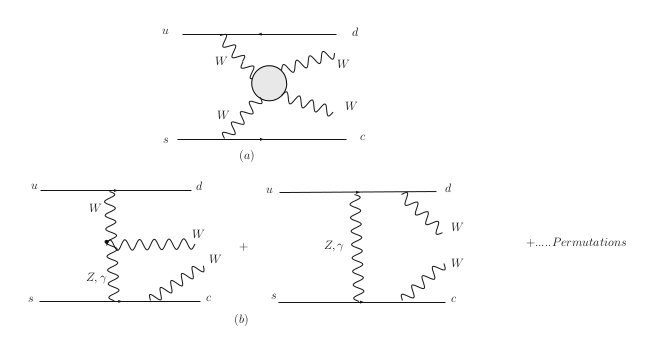
\includegraphics[width=16.0cm,height=8cm]{figures/VBS/ww_scat.png}
		\caption{Main diagram topologies for the process $us \rightarrow cdW^+W^-$}
		\label{wwscat}
	\end{center}
\end{figure} 
Thus to study WW scattering at the LHC, we have to find out the ways of separating the genuine scattering contribution from the other ``Bremsstrahlung" contributions, which is no mean task. 
\begin{comment}
\subsection{Backgrounds}
It is important to understand the first inherent background, and device cuts which may enhance the signal. Generally, the backgrounds in this case are of two types:
\begin{enumerate}
	\item Bremsstrahlung processes - these are processes where the vector bosons are radiated by quark or anti-quark partons, and which do not contribute to VV scattering.
	\item Processes which fake a VV final state.
\end{enumerate}
 The second background is crucial to take care of, otherwise we do not know if we are observing a VV pair in the final state or not.

Background processes are $q\bar{q} \rightarrow W^+W^-X$, $gg \rightarrow W^+W^-X$, $t\bar{t}+jet$, with top decays giving $W^+W^-$ pair. Electroweak-\gls{qcd} process $W^+ +jets$ can mimic the signal when the invariant mass of the two jets is around $m_w$. There is a potential background from \gls{qcd} processes $q\bar{q},gg\rightarrow t\bar{t}X,$  $Wt\bar{b}$ and $(t\bar{t} + jets)$, in which a W can come from the decay of $t$ or $\bar{t}$. W boson pairs produced from the intrinsic electroweak process $q\bar{q}\rightarrow q\bar{q}W^+W^-$ tend to be transversely polarised. 


Compared to the dileptonic channel, the well-known challenge for the semileptonic $W_LW_L$ scattering is the contamination from \gls{qcd} backgrounds. However, the semileptonic channel is still appealing because it yields much more signal events and enables reconstruction of the W momenta and thus important kinematics such as the WW invariant mass.\cite{arXiv:WWscat-WjetTag} 
\end{comment}
\subsection{Signal \& Background Details}
I have started working on WW scattering measurement at the {cms} experiment \cite{paper:JINST:CMSCollaboration}. The {lhc} is currently going through shutdown after running for 3 years at 7 \& 8 TeV centre of mass energy. {cms} experiment collected about $5fb^{-1}$ of data at 7TeV and $20fb^{-1}$ data at 8TeV. The {lhc} is scheduled to start operating at 13 and/or 14 TeV energy form next year. Since the WW scattering measurement prospects will increase considerably at higher energies so we need to be prepared fully to perform this measurement once LHC starts delivering the data. Currently I am working on the development of necessary techniques needed to discriminate the WW signal from the other similar SM backgrounds.\\ {\large \bf Signal :} Since the channel on which I work is $qq\rightarrow qqW_LW_L \rightarrow l\nu jjjj$. So, my signal in first stage contains 2 jets that are coming from hadronic decay of quarks and two longitudinal component of W. And in last stage it contains one lepton, 4 jets (2 coming from hadronic decay of quarks and 2 coming from hadronic decay of $W_L$) and one neutrino which constitute missing energy. Here, lepton includes electron and muon.\\{\large \bf Background :} The processes which can fake the final state are known as background. It is important to understand the first inherent background, and device cuts which may enhance the signal. Generally, the backgrounds in this case are of two types:
\begin{enumerate}
	\item Bremsstrahlung processes - these are processes where the vector bosons are radiated by quark or anti-quark partons, and which do not contribute to VV scattering.
	\item Processes which fake a VV final state.
\end{enumerate}
 The second background is crucial to take care of, otherwise we do not know if we are observing a VV pair in the final state or not.
All possible backgrounds are:
	\begin{enumerate}
		\item {\bf W+Jets :} Most dominating background. W decays to $l\nu $
		\item {\bf Drell-Yan $Z/\gamma*$+ Jets :} $Z/\gamma*$ decays to $l^+l^-$ and we mismeasure one l because of acceptance or inefficiency effects, gives missing energy.
		\item {\bf WW :} This is irreducible background for analysis.
		\item {\bf WZ :} Z decays to $l^+l^-$ and we mismeasure one $l$ giving missing energy. And W decays hadronically.
		\item {\bf ZZ :} One Z decays hadronically and another leptonically and we miss one $l$.
		\item {\bf $t\bar{t}$ Jets :} Top quark always decays to one b quark and one W boson. So, $t\bar{t} \rightarrow bWbW \rightarrow bl\nu bl\nu$, if we mismeasure one $l$ and and b quark forms jet.
		\item {\bf Single top production :} Here $t\rightarrow bW \rightarrow bl\nu $, and 3 fake jet is reconstructed or we get some form ISR or FSR.
	\end{enumerate}

\subsection{Separating Signal form various Background}
The central issue for the experimental detection of WW scattering is to separate the signal among all the various backgrounds. The signal is the {vbf} diagrams, each of the initial quarks radiates a W/Z boson, which further scatters into the final state W/Z bosons. The unique feature of this process is that the scattered quark is very energetic, carrying almost all the energy of the incoming quark and very forward. Furthermore, if we demand the leptonic decays of the W and Z bosons, there will be very little hadronic activities in the central rapidity region. Therefore, the signature includes
	\begin{enumerate}
		\item the appearance of two energetic forward jets with large spatial separation, and 
		\item the leptonic decay products of the W or Z bosons are enhanced at the large invariant mass region.
	\end{enumerate}
Based on these features we can start the analysis by imposing the following experimental cuts for the two jets in selecting the VBF events:
	\begin{itemize}
		\item Two tagging jets $j_1,j_2$ with \begin{equation} 2<|\eta|<5,~ p_T>25GeV,~E>340GeV,~and~\eta_{j1}.\eta_{j2}<0 \end{equation} Where $\eta$ is the rapidity of either jet,\\ $p_T$ is the transverse momentum,\\ E is the energy, \\ $\eta_{j1} ~ \& ~ \eta_{j2}$ are the rapidities of jet 1 and jet 2 respectively.
		\item $p^w_T>350GeV$ for both W's. Here $p^w_T$ is the transverse momentum of W boson.
		\item The two partons from the W decay have a $p_T$ ratio $>$ 0.1 (lower/higher), for both W's.
		\item $m_{ww}$ ( mass of both W boson) $>850GeV$.
	\end{itemize}
These cuts basically suppress the electroweak backgrounds.
Another, additional cuts or taggings are:
	\begin{itemize}
		\item W-jet tagging : Basically done on the basis of Jet substructure. Here the W is highly boosted and hence when W decays hadronically then the two jets will generally merge into one. So, the Jet substructure will help to improve signal/background. The differences between the boosted W-jet and a QCD jet in distinguishing them is listed below : \cite{paper:arXiv:WWscat-WjetTag}. 
			\begin{itemize}
			\item W jet contains two hard subjets (i.e., subregions where the jet energy is concentrated), originated from the two quarks in the W decay, while a QCD jet usually has only one hard subjet.
			\item The W boson is a color singlet particle, consequently all QCD radiation from the decay of a boosted W is confined in a small cone around the W momentum direction. On the other hand, a QCD jet is initiated from a color triplet or octet, which is color-connected to the beam or the other side of the event. Therefore, the radiation of a QCD jet is usually much more diffuse.
			\end{itemize}
		\item b-jet tagging
		\item mass window cut
	\end{itemize}
The cuts for leptonic decay mode of W is :
	\begin{itemize}
	\item leptons should be isolated.
	\item $p_T>20GeV$, $|\eta|<2.4$
	\item Sum of the transverse energies around the lepton in a cone $\Delta R = \sqrt{\Delta \phi^2 + \Delta \eta^2} <0.3$ must satisfy $\sum E_T<0.14p_T^{lep}.$

	\end{itemize}
Also, we can try any new variable or cuts by analysing the improvement in signal/background ratio.


\begin{comment}
\begin{equation}
	E_{T_{j1,j2}}>30GeV,~~|\eta_{j1,j2}|<4.7,~\Delta \eta_{12}=|\eta_{j1}-\eta_{j2}|>3.5,~\eta_{j1}\eta_{j2}<0,
\end{equation}
Where $E_{T_{j1,j2}}$ and $\eta_{j1,j2}$ are the transverse energies and pseudo-rapidities respectively of the two forward jets, and
\begin{equation}
	M_{jj}>500~GeV
\end{equation}
on their invariant mass $M_{jj}$ at $\sqrt{s}=8TeV$.
The cuts for the leptonic decay modes $W\rightarrow l\nu_l$ for $W^+W^-$ is given below:
\begin{equation}
	p_{T_l}>100GeV,~|\eta_l|<2,~M_{l^+l^-}>250GeV
\end{equation}
Compared to the dileptonic channel, the well-known challenge for the semileptonic $W_LW_L$ scattering is the contamination from \gls{qcd} backgrounds. However, the semileptonic channel is still appealing because it yields much more signal events and enables reconstruction of W momenta and thus important kinematics such as the WW invariant mass. 


To reject major \gls{qcd} backgrounds and boos the longitudinal fraction of the W's central jet veto and tagging jets requirements are used. There persistent background is W+jets where W decays leptonically. In a signal event, the hadronically decaying W is highly boosted at high energies, thus behaves as a single jet in a collider detector, which we call a W jet. In order to reject the W+jets background, it is essential to distinguish a W jet from a \gls{qcd} jet initiated from a quark or a gluon.

%\subsection{Experimental Work}


\subsection{Analysis Strategy}
We can divide our analysis mainly in three steps:
	\begin{itemize}
		\item Preporcessing : Here the raw data that contains only hits and energy deposit information is stored and first converted into RECO format and then AOD format. This AOD data mainly contains reconstructed objects like tracks, vertices, jets, electrons, muons, etc.
		\item Processing : First, We run PatTuple on the AOD data, then Ntuple and finally we create RDTrees.
		\item Analysis : Finally we start looking various distributions,applying the cuts and other methods to improve signal and background ratio, then doing MC/Data comparision, etc. according to our need.
	\end{itemize}
Some distribution like $ E_T,p_T, \eta, \phi$, etc for all background is shown below:
\end{comment}
